\documentclass[11pt]{beamer}
\usetheme{metropolis}

\usepackage[utf8]{inputenc}
\usepackage[english]{babel}
\usepackage{listings}
\usepackage{color}
\usepackage{csquotes}
\usepackage{graphicx}
\usepackage{tabularx}
\usepackage[linesnumbered,ruled,vlined]{algorithm2e}
\usepackage[backend=bibtex,style=ieee]{biblatex}
\usepackage{mathtools}
\usepackage{bm}

\makeatletter
\def\beamer@framenotesbegin{% at beginning of slide
    \usebeamercolor[fg]{normal text}
    \gdef\beamer@noteitems{}%
    \gdef\beamer@notes{}%
}
\makeatother

\definecolor{mygreen}{rgb}{0,0.6,0}
\definecolor{mygray}{rgb}{0.5,0.5,0.5}
\definecolor{mymauve}{rgb}{0.58,0,0.82}

\lstset{ %
    backgroundcolor=\color{white},   % choose the background color
    basicstyle=\footnotesize,        % size of fonts used for the code
    breaklines=true,                 % automatic line breaking only at whitespace
    captionpos=b,                    % sets the caption-position to bottom
    commentstyle=\color{mygreen},    % comment style
    escapeinside={\%*}{*)},          % if you want to add LaTeX within your code
    keywordstyle=\color{blue},       % keyword style
    stringstyle=\color{mymauve},     % string literal style
}

\newcommand{\vect}[1]{\boldsymbol{\mathbf{#1}}}

\bibliography{bibliography.bib} 

\author{Mario Tambos}

\title{Hidden Markov Models}
\subtitle{Introduction to Computational Genomics Seminar}
\institute{M.sc. Computer Science @ TU Berlin}

\date{\today}

\begin{document}
	\maketitle
	\section{Contents}
	\begin{frame}
		\frametitle{Contents}
        \begin{itemize}
            \item The Setting - Nucleic and Amino Acid Chains
            \item Tasks
            \item Hidden Markov Models
            \item Example - Segmenting the Lambda Phage Genome
            \item Case Study - Olfactory Receptors
            \item Notes and Attributions
            \item Questions?
            \item References
        \end{itemize}
	\end{frame}
	\section{The Setting - Nucleic and Amino Acid Chains}
    \subsection{What are we working with?}
    \begin{frame}
        \frametitle{What are we working with?}
        Objects of study:
        \begin{itemize}
            \item Genes
            \item Proteins
        \end{itemize}
        Main question:
        \begin{quote}
            What can we say about the function of an object by looking at it's structure?
        \end{quote}
    \end{frame}

    \subsection{How are the objects represented?}
    \begin{frame}
        \frametitle{How are the objects represented?\quad i}
        Representation:
        \begin{itemize}
            \item Sequences of nucleic and amino acids
            \item Strings of characters
            \item Every character is a an nucleic acid (genes, 4 charachters: CGAT\footnote{In DNA} or CGAU\footnote{In RNA}) \cite{cristianini2006introduction},
            \item or an amino acid (proteins, 20 characters\footnote{Many more exist, but only 20 are present in DNA}) \cite{cristianini2006introduction}
        \end{itemize}
    \end{frame}
    \begin{frame}
        \frametitle{How are the objects represented?\quad ii}
        Examples:
        \begin{itemize}
            \item (Partial) Gene \cite{finn2016pfam}:\\
            \texttt{ATGAGCACAAAAAAGAAACCATTAACACAAGAGCAGCTTGAGGACG}[...]
            \item (Partial) Protein \cite{finn2016pfam}:\\
            \texttt{MGRPVSTFLIVIIGVSLAYADIYLHNMRGSNNC}[...]
        \end{itemize}
    \end{frame}

    \section{Tasks}
    \subsection{Common Tasks}
    \begin{frame}
        \frametitle{Common Tasks}
        \begin{itemize}
            \item Sequence multiple alignment
            \item Sequence segmentation
            \item Prediction of function
            \item Gene finding
        \end{itemize}
    \end{frame}

    \subsection{Assumptions}
    \begin{frame}
        \frametitle{Assumptions}
        \begin{itemize}
            \item Representation is powerful enough
            \item There's some phenomenon not directly visible (e.g., the function we're trying to predict) that affects the features we observe in the representation
        \end{itemize}
    \end{frame}
    
    \section{Hidden Markov Models}
    \subsection{Description}
    \begin{frame}
        \frametitle{Description\footnote{Unless otherwise specified, everything that follows is based on \cite{cristianini2006introduction}}}
        \begin{itemize}
            \item Probabilistic generative model
            \item Generalization of mixture models
            \item Two types of processes:
            \begin{itemize}
                \item State change (unobserved) $\rightarrow$ $h^{(t)}$ depends \textbf{only} on $h^{(t-1)}$
                \item Emission (observed) $\rightarrow$ $s^{(t)}$ depends \textbf{only} on $h^{(t)}$
                \item States are always discrete and obey the Markov property
                \item Emissions can be discrete or continuous
            \end{itemize}
        \end{itemize}
    \end{frame}

    \subsection{Example - Two Dice}
    \begin{frame}
        \frametitle{Example - Two Dice\quad i}
        \begin{itemize}
            \item Two dice, one loaded, one fair; otherwise identical
            \item Someone picks one die at random, throws it, and we record the result
            \item The process could have parameters as follows:
        \end{itemize}
        \centering
        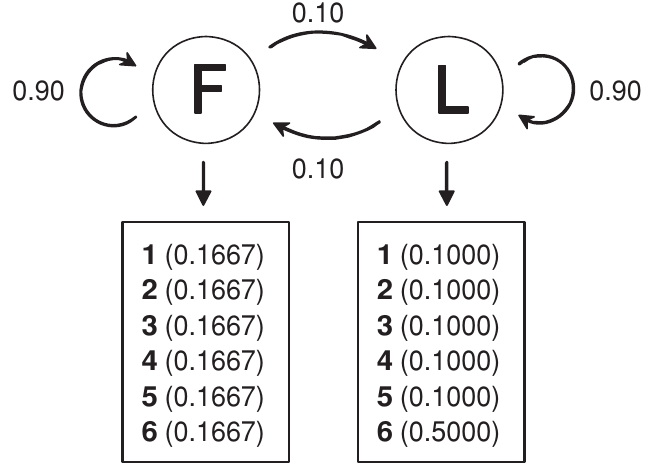
\includegraphics[height=0.6\textheight]{images/two_dice_params.png}
    \end{frame}
    
    \begin{frame}
        \frametitle{Example - Two Dice\quad ii}
        \begin{itemize}
            \item Given the sequence:\\
            \texttt{s = 4553653163363555133362665132141636651666}
            \item What's the sequence's probability?
            \item What die generated each number?
            \item HMM answers \footnote{Partial. Rows: seq. prob.; prob. of fair; prob. of loaded; seq.; state (1$\rightarrow$fair, 2$\rightarrow$loaded)}:
        \end{itemize}
        \centering
        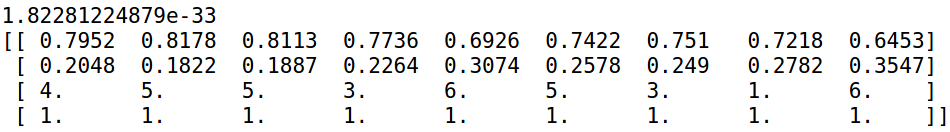
\includegraphics[scale=0.3]{images/two_dice_results.png}
    \end{frame}
    
    \subsection{Formal definition}
    \begin{frame}
        \frametitle{Formal definition\quad i}
        The parameters of a Hidden Markov Model \cite{Bishop2006}, with hidden states $h \in \mathcal{H};|\mathcal{H}|=N$, are a triplet:
        $$
            \vect{\theta} = (\vect{\pi}, \vect{T}, \phi)
        $$
        where:
        \begin{itemize}
            \item $\vect{\pi} \in [0,1]^N$: initial probabilities of the states $s_1$
            \item $\vect{T} \in [0,1]^{N\times N}$: matrix of elements $T_{ij}$ of transition probabilities $p(h_j|h_i)$
            \item $\phi$: emission distribution model $p(s_j|h_i)$ of observing $s_j$ in state $h_i$
        \end{itemize}
    \end{frame}
    
    \begin{frame}
        \frametitle{Formal definition\quad ii}
        The joint probability distribution over $h$ and $s$, both of length $L$, is \cite{Bishop2006}:
        $$
        p(\vect{s}, \vect{h}|\vect{\theta}) = p(h_1|\pi)\left[\prod_{l=2}^L p(h_l|h_{l-1}, \vect{T})\right]\prod_{k=2}^L p(s_k|h_k, \phi)
        $$
     \end{frame}
   
    \subsection{Multinomial HMM}
    \begin{frame}
        \frametitle{Multinomial HMM}
        \begin{itemize}
            \item Observations $s \in \mathcal{S}, |\mathcal{S}|=M$\footnote{Elements of $\mathcal{S}$ are sometimes called \emph{symbols}}
            \item Instead of $\phi$, we have a matrix $E \in [0,1]^{N\times M}$
            \item $E_{ij}$ $\rightarrow$ emission probability $p(s_j|h_i)$
            \item Joint probability:
            \begin{align*}
            p(\vect{s}, \vect{h}|\vect{\theta}) &= p(h_1|\pi)\left[\prod_{l=2}^L p(h_l|h_{l-1}, \vect{T})\right]\prod_{k=2}^L p(s_k|h_k, \vect{E})\\
                                                      &= \pi_{h_1} \left[\prod_{l=2}^L \vect{T}_{h_{l-1},h_l}\right] \prod_{k=2}^L \vect{E}_{h_k,s_k}
            \end{align*}
        \end{itemize}
    \end{frame}
   
   \subsection{Useful Probabilities}
   \begin{frame}
       \frametitle{Useful Probabilities}
       \begin{itemize}
           \item Probability of a certain sequence of hidden states
           $$
           p(\vect{h}|\vect{\theta}) = p(h_1|\pi)\prod_{l=2}^L p(h_l|h_{l-1}, \vect{T}) = \pi_{h_1} \prod_{l=2}^L \vect{T}_{h_{l-1},h_l}
           $$
           \item Probability of a certain sequence of symbols given a certain sequence of hidden states
           $$
           p(\vect{s}|\vect{h},\vect{\theta}) = \prod_{k=2}^L p(s_k|h_k, \vect{E}) = \prod_{k=2}^L \vect{E}_{h_k,s_k}
           $$
        \end{itemize}
    \end{frame}
    
   \subsection{Usual Tasks}
   \begin{frame}
       \frametitle{Usual Tasks\quad i}
       \begin{itemize}
           \item Find probability of a certain sequence of symbols $\vect{s}$ with unknown hidden states
           $$
           p(\vect{s}|\vect{\theta}) = \sum_{\forall \vect{h}_j \in \mathcal{H}^L}p(\vect{s},\vect{h}_j|\vect{\theta})
           $$
           \item Find most likely sequence of states, given a sequence of symbols $\vect{s}$
           $$
           \vect{h}^* = \arg \max_{\forall \vect{h}_j \in \mathcal{H}^L} p(\vect{s},\vect{h}_j|\vect{\theta})
           $$
        \end{itemize}
    \end{frame}

   \begin{frame}
       \frametitle{Usual Tasks\quad ii}
           Both seem to be $O(e^L)$
           
           $\rightarrow$ we need some way of making these calculations tractable

           $\rightarrow$ exploit independences in the model

           $\rightarrow$ $ML(\vect{h}^{(t)})$ can be written as $f\left[ML(\vect{h}^{(t-1)})\right]$ (sim. for $\vect{s}^{(t)}$)

           $\rightarrow$ \emph{Viterbi} and \emph{Forward} algorithms
    \end{frame}
    
   \subsection{Viterbi Algorithm}
   \begin{frame}
       \frametitle{Viterbi Algorithm}
       Calculates the ML of the hidden states' sequence $\vect{h}^*$, given $\vect{s}$
       \smaller{
           \begin{algorithm}[H]
               \DontPrintSemicolon
               \KwData{Sequence $\vect{s}=(s_1, \dots, s_L)$; model $\vect{\theta}=(\vect{\pi},\vect{T},\vect{E})$}
               \KwResult{$\left[p\left(\vect{s},\vect{h}^*\right),\vect{h}^*\right]$, where $\vect{h}^*$ is the most likely states' sequence}
               \Begin{
                   $\vect{V} \coloneqq \vect{0}^{N\times (L+1)}$\;
                   $\vect{pointer} \coloneqq \vect{0}^{N\times L}$\;
                   $\vect{V}_{0,0} \coloneqq 1$ \tcp*{In \cite{Bishop2006}: $\vect{V}_{k,0} \coloneqq \vect{\pi}_k \vect{E}_{k,\vect{s}_i}$}
                   \For{$i=1:L$}{
                       \For{$l=1:N$}{
                           $\vect{V}_{l,i} \coloneqq \vect{E}_{l,\vect{s}_i}\max_k \left[\vect{V}_{k,i-1}\vect{T}_{k,l}\right];$\;
                           $\vect{pointer}_{i,l} \coloneqq \arg\max_k \left[\vect{V}_{k,i-1}\vect{T}_{k,l}\right]$	\;
                       }
                   }
                   $p\left(\vect{s},\vect{h}^*\right) \coloneqq \max_k \vect{V}_{k,L}$\;
                   $\vect{h}^* \coloneqq \vect{0}^L$\;
                   $\vect{h}^*_L \coloneqq \arg\max_k\vect{V}_{k,L}$\;
                   \For{$i=(L-1):1$}{
                       $\vect{h}^*_i \coloneqq \vect{pointer}_{i,\vect{h}^*_{i}} $\;
                   }
               }
           \end{algorithm}
        }
    \end{frame}
    
    \subsection{Forward Algorithm}
    \begin{frame}
        \frametitle{Forward Algorithm}
        Calculates the probability of the sequence $\vect{s}$ under the model
        \smaller{
            \begin{algorithm}[H]
                \DontPrintSemicolon
                \KwData{Sequence $\vect{s}=(s_1, \dots, s_L)$; parameters $\vect{T},\vect{E}$}
                \KwResult{$p(\vect{s})$}
                \Begin{
                    $\vect{F} \coloneqq \vect{0}^{N\times (L+1)}$\;
                    $\vect{F}_{0,0} \coloneqq 1$\tcp*{In \cite{Bishop2006}: $\vect{F}_{k,0} \coloneqq \vect{\pi}_k \vect{E}_{k,\vect{s}_i}$}
                    \For{$i=1:L$}{
                        \For{$l=1:N$}{
                            $\vect{F}_{l,i} \coloneqq \vect{E}_{l,\vect{s}_i}\sum_{k=1}^{N} \left[\vect{F}_{k,i-1}\vect{T}_{k,l}\right];$\;
                        }
                    }
                    $p(\vect{s}) \coloneqq \sum_{k=1}^{N} \vect{F}_{k,L}$\;
                }
            \end{algorithm}
        }
    \end{frame}

    \subsection{Learning \texorpdfstring{$\vect{\theta}$}{TEXT}}
    \begin{frame}
        \frametitle{Learning $\vect{\theta}$}
        \begin{itemize}
            \item Problem: learn $\vect{\theta}$ from $\vect{s}$ only ($\vect{h}$ unknown)
            \item No closed-form solution
            \item Can have local maxima
            \item \cite{cristianini2006introduction} only gives a high-level outline: use EM
            \item \cite{Bishop2006} provides an in depth explanation of how to proceed
        \end{itemize}
    \end{frame}
    
    \section{Example - Segmenting Lambda Phage Genome}
    \begin{frame}
        \frametitle{Example - Segmenting Lambda Phage Genome\quad i}
        \begin{itemize}
            \item Problem: Segment the genome into CG-rich and AT-rich blocks
            \item Use HMM with \texttt{ATCG} as symbols and \texttt{CG-rich} and \texttt{AT-rich} as hidden states
            \item After training with EM, we obtain the following $\vect{T}$ and $\vect{E}$:
        \end{itemize}
        \centering
        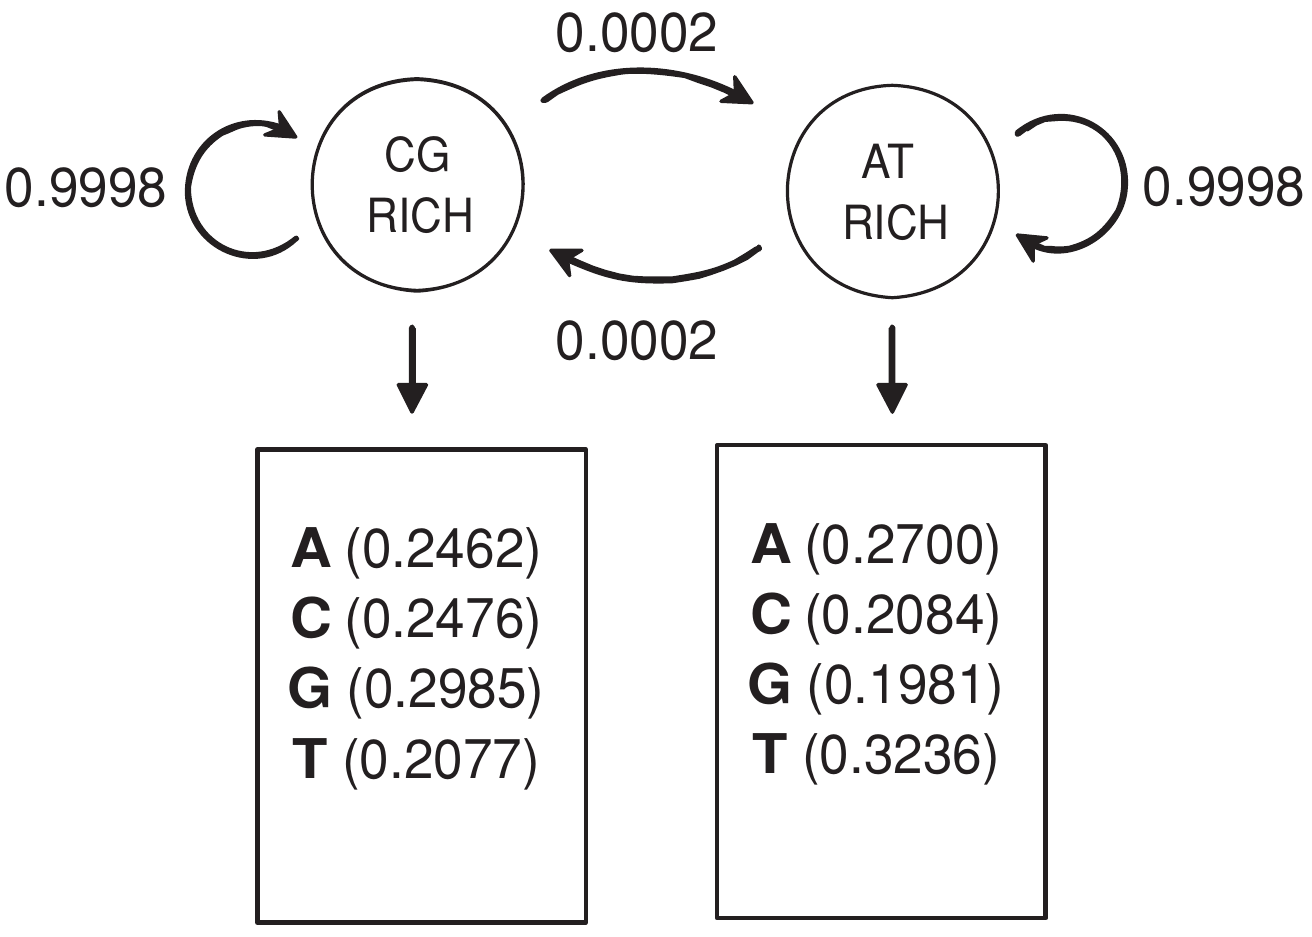
\includegraphics[scale=0.2]{images/lp_seg_params.png}
    \end{frame}

    \begin{frame}
        \frametitle{Example - Segmenting Lambda Phage Genome\quad ii}
        With those parameters + the Viterbi algorithm we get:
        \centering
        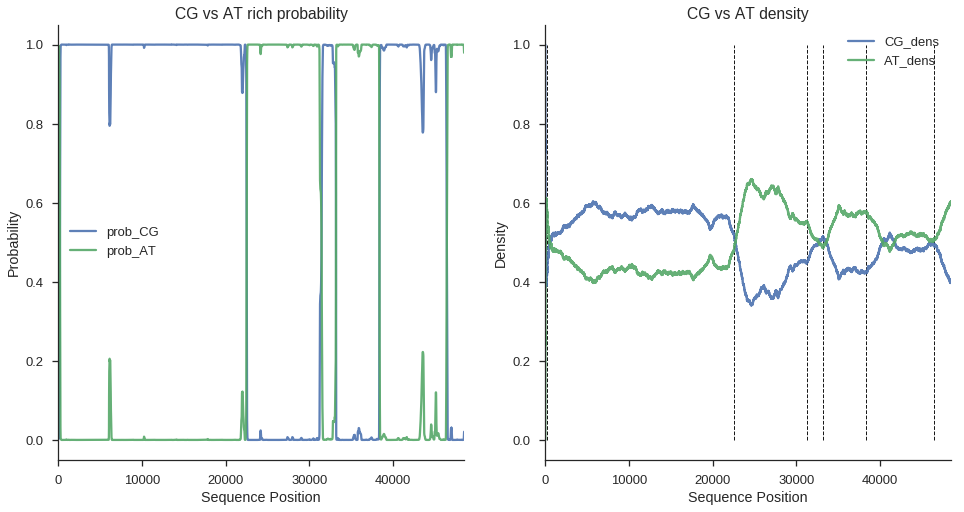
\includegraphics[width=\textwidth]{images/lp_seg_results.png}
    \end{frame}
    
   
    \section{Case Study - Olfactory Receptors}
    \begin{frame}
        \frametitle{Case Study - Olfactory Receptors}
        \begin{itemize}
            \item Data: set of amino acid's sequences (proteins)
            \item Given a single protein, answer two questions:
            \begin{itemize}
                \item What sections are hydrophobic, what are hydrophilic?
                \item Does the protein belong to a known family?
            \end{itemize}
        \end{itemize}
        \colorbox{lightgray}{
            \centering
            \begin{minipage}{0.81\textwidth}
                \small{\texttt{MAMDNVTAVF QFLLIGISNY PQWRDTFFTL VLIIYLSTLL GNGFMIFLIH FDPNLHTPIY
                        FFLSNLSFLD LCYGTASMPQ ALVHCFSTHP YLSYPRCLAQ TSVSLALATA ECLLLAAMAY
                        DRVVAISNPL RYSVVMNGPV CVCLVATSWG TSLVLTAMLI LSLRLHFCGA NVINHFACEI
                        LSLIKLTCSD TSLNEFMILI TSIFTLLLPF GFVLLSYIRI AMAIIRIRSL QGRLKAFTTC
                        GSHLTVVTIF YGSAISMYMK TQSKSSPDQD KFISVFYGAL TPMLNPLIYS LRKKDVKRAI
                        RKVMLKRT}}
            \end{minipage}
        }

    \end{frame}
    
    \subsection{Identifying Hydrophobic Blocks}
    \begin{frame}
        \frametitle{Identifying Hydrophobic Blocks\quad i}
        \begin{itemize}
            \item Each symbol has its own h-phobicity index
            \item Interested in h-phobicity index of blocks
            \item Approach: train an HMM on all proteins with:
            \begin{itemize}
                \item two hidden states (\texttt{hydrophilic}/\texttt{hydrophobic})
                \item 20 symbols (one for each amino acid)
            \end{itemize}
            \item Very similar to the CG-heavy block detection.
        \end{itemize}
        
    \end{frame}

    \begin{frame}
        \frametitle{Identifying Hydrophobic Blocks\quad ii}
        After training with EM, we obtain the following $\vect{T}$ and $\vect{E}$:
        \centering
        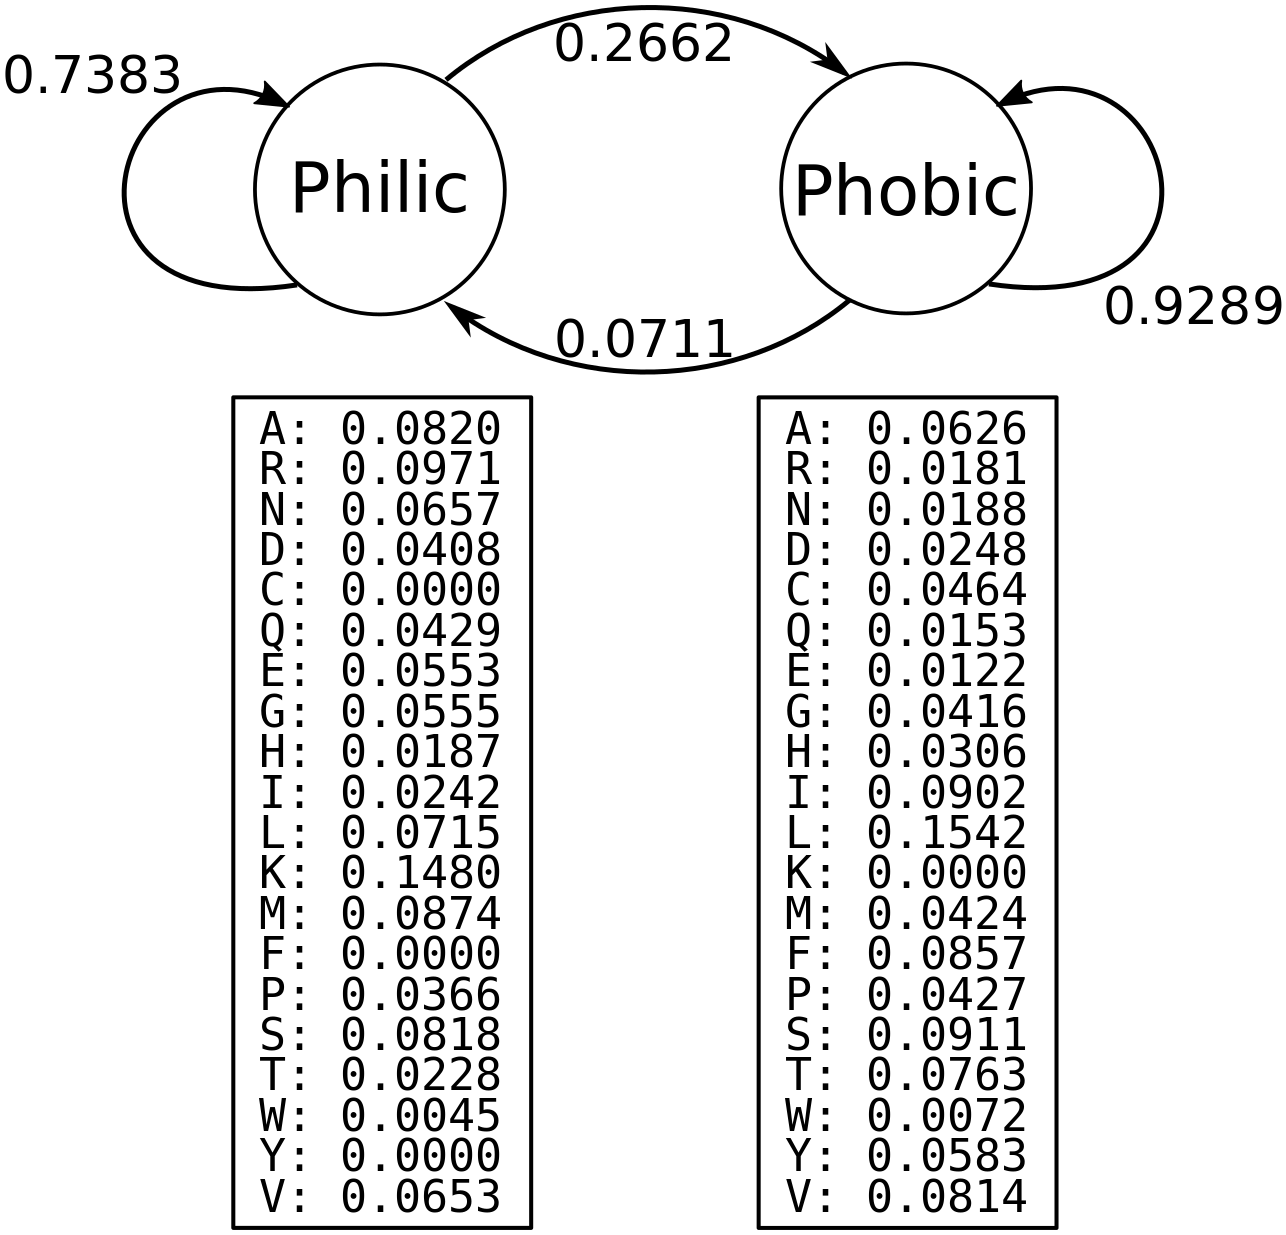
\includegraphics[height=0.8\textheight]{images/or_hydro_params.png}
    \end{frame}

    \begin{frame}
        \frametitle{Identifying Hydrophobic Blocks\quad iii}
        With those parameters + the Viterbi algorithm we get\footnote{Hydrophobicity calculated using Kyte \& Doolittle index \cite{KYTE1982105}}:
        \centering
        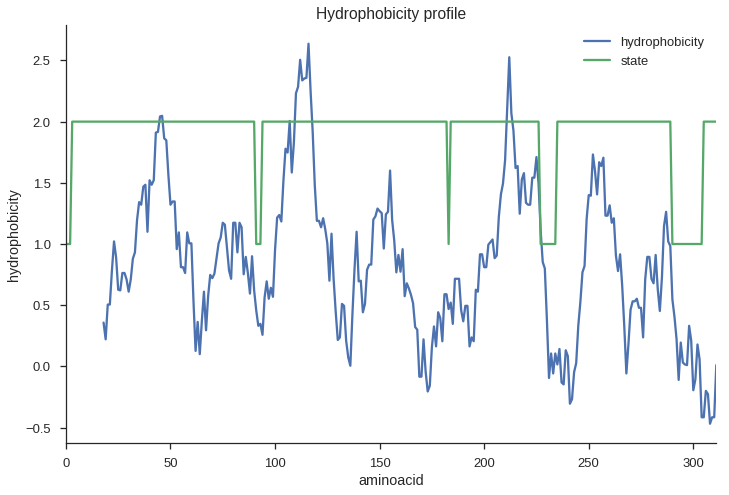
\includegraphics[height=0.7\textheight]{images/or_hydro_results.png}
    \end{frame}

    \subsection{Matching to a Protein Family}
    \begin{frame}
        \frametitle{Matching to a Protein Family\quad i}
        \begin{itemize}
            \item Different proteins have different amino acid representations (even in length)
            \item All proteins in a family share some common structure
            \item Assumption: members of a family will be better aligned among themselves than with members of other families
        \end{itemize}
    \end{frame}
    
    \begin{frame}
        \frametitle{Matching to a Protein Family\quad ii}
        Approach:
        \begin{itemize}
            \item Use a set of protein sequence alignments to train an HMM
            \item Symbols are the usual amino acid's alphabet
            \item One hidden state for each symbol match, insert and delete
            \begin{itemize}
                \item e.g., an alignment 20 characters long trains an HMM with 60 hidden states
            \end{itemize}
            \item Left-to-right HMM: $T_{j, k} = 0;\forall k<j$
        \end{itemize}
        \centering
        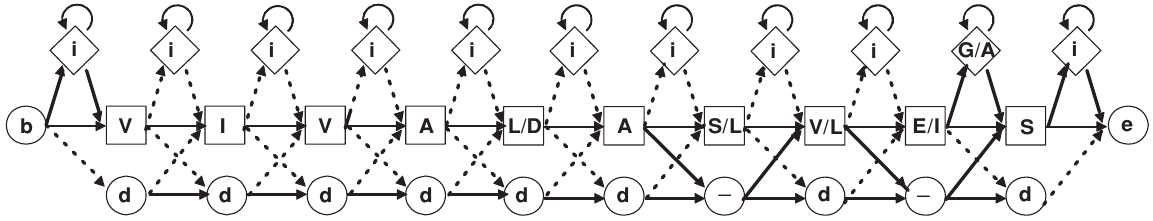
\includegraphics[width=\textwidth]{images/phmm_example.png}
    \end{frame}
    
    \begin{frame}
        \frametitle{Matching to a Protein Family\quad iii}
        \begin{itemize}
            \item Setup known as Profile HMM (pHMM)
            \item Suppose pHMM $\mathcal{M}$ trained in family $\mathcal{F}$, and new sequence $\vect{s}$
            \begin{itemize}
                \item $p(\vect{s}|\mathcal{M})$ high $\rightarrow \vect{s}\in \mathcal{F}$ 
                \item $\vect{h}^*$ obtained with the Viterbi algorithm $\rightarrow$ "virtual" alignment of $\vect{s}$ with all members of $\mathcal{F}$
            \end{itemize}
        \end{itemize}
    \end{frame}
    
    \begin{frame}
        \frametitle{Matching to a Protein Family\quad iv}
        pHMM setup:
        \begin{itemize}
            \item Alignment length: 268
            \item Hidden states
            \begin{itemize}
                \item Two special begin states $B$ and $I_0$:
                \begin{align*}
                B \rightarrow M_1; &B \rightarrow I_0; B \rightarrow D_1;\\
                I_0 \rightarrow M_1; &I_0 \rightarrow I_0\\
                \end{align*}
                \item 268 $M$, $I$ and $D$ states:
                \begin{align*}
                M_t \rightarrow M_{t+1} &; M_t \rightarrow I_t; M_t \rightarrow D_{t+1}\\
                I_t \rightarrow M_{t+1} &; I_t \rightarrow I_t \\
                D_t \rightarrow M_{t+1} &; D_t \rightarrow D_{t+1} \\
                \end{align*}
                \item All others are 0
            \end{itemize}
        \end{itemize}
    \end{frame}
    
    \begin{frame}
        \frametitle{Matching to a Protein Family\quad v}
        \begin{itemize}
            \item Experiment objective: check that a pre-trained pHMM correctly identified members of the family.
            \item Hypothesis: the pHMM will provide higher scores to members than to shuffled versions of themselves.
            \end{itemize}
    \end{frame}
    
    \begin{frame}
        \frametitle{Matching to a Protein Family\quad vi}
        Original vs shuffled sequences' alignment scores
        \centering
        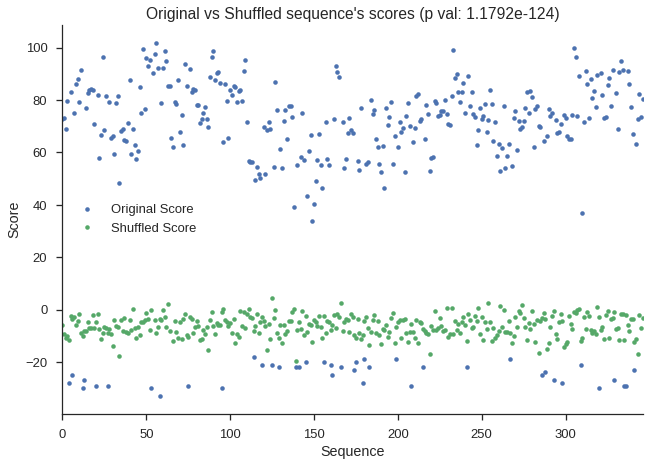
\includegraphics[width=\textwidth]{images/or_align_results.png}
    \end{frame}

    
    \begin{frame}
        \frametitle{Matching to a Protein Family\quad vii}
        Original vs shuffled sequences' predicted alignments
        \centering
        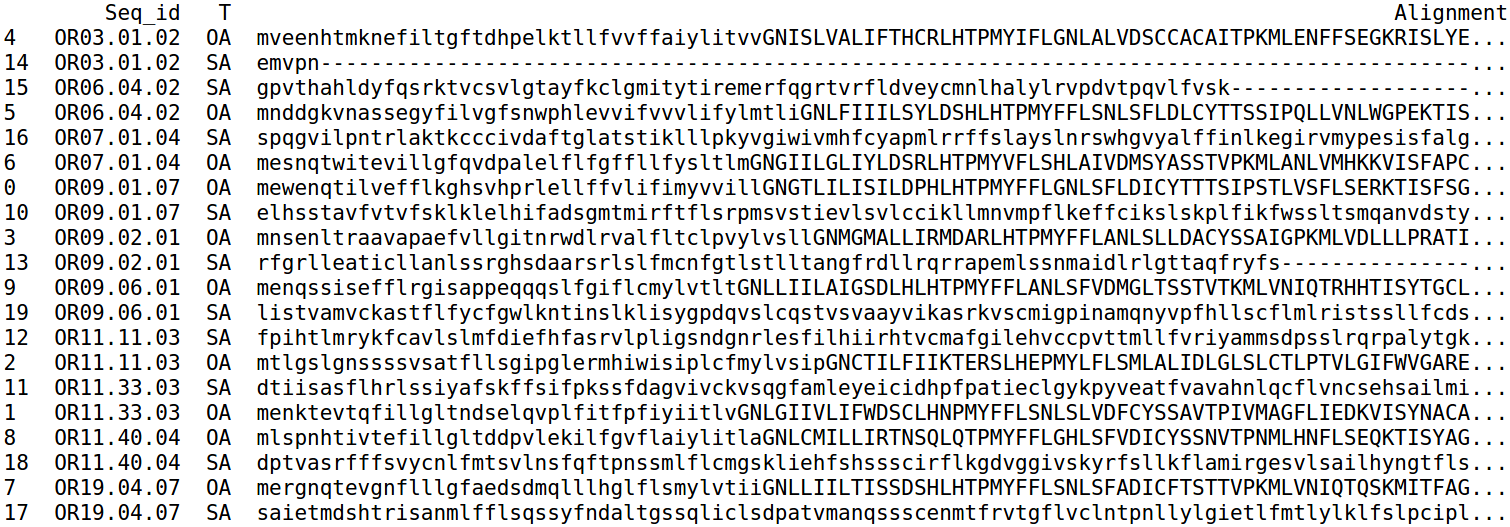
\includegraphics[width=\textwidth]{images/or_align_sample.png}
    \end{frame}

    \section{Notes and Attributions}
    \begin{frame}
        \frametitle{Notes and Attributions}
        \begin{itemize}
            \item Code written in \texttt{Python}, using the packages \texttt{biopython}, \texttt{hmmlearn}, \texttt{matplotlib}, \texttt{numpy}, \texttt{pandas}, \texttt{requests} and \texttt{seaborn}
            \item For the Olfactory Receptors section, the \texttt{hmmer} \cite{hmmer} program suite was used
            \item Data and model for the Olfactory Receptors section were obtained from \cite{finn2016pfam}
            \item All third-party images were taken from \cite{cristianini2006introduction}
            \item Talk written in \LaTeX\ using \texttt{TeXstudio}
        \end{itemize}
    \end{frame}

    \section{Questions?}
    

    \begin{frame}[t,allowframebreaks]{Roman}
        \frametitle{References}
        \printbibliography
    \end{frame}
\end{document}